\section{Sequence-to-sequence models}

RNNs and their more advanced variant, LSTMs, proved to be so powerful that they quickly became the go-to solution for sequence-to-sequence (seq2seq) tasks—problems where the input is a sequence of data and the output is another sequence. 
One of the most prominent applications of seq2seq models is machine translation, where an input sentence in one language is translated into another language.
To build a translation model using LSTMs, two distinct RNN-based components are typically trained:
\begin{itemize}
    \item \textit{Encoder}: this component processes the input sequence and generates a compact representation of the entire sequence. 
        Essentially, it encodes the meaning of the input into a fixed-size vector.
    \item \textit{Decoder}: takes this encoded representation as its starting point and generates the output sequence word by word. 
        It essentially decodes the meaning captured by the encoder into the target language or desired output format.
\end{itemize}
\begin{figure}[H]
    \centering
    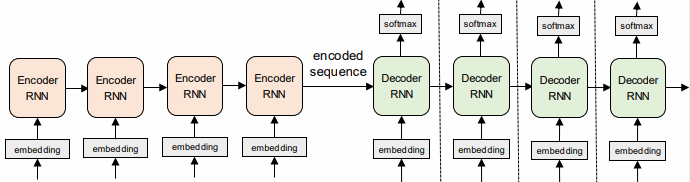
\includegraphics[width=0.5\linewidth]{images/nlp3.png}
    \caption{Sequence to sequence}
\end{figure}
\noindent This encoder-decoder framework revolutionized the field of NLP and set new state-of-the-art performance benchmarks across a wide range of tasks.
In fact, many NLP problems can be framed as seq2seq tasks.

One major issue is that the encoder must compress all the information from the input sequence into a single fixed-size vector, which is then passed to the decoder. 
This bottleneck can lead to information loss, especially when dealing with long sequences.
As a result, the decoder might struggle to generate accurate translations or outputs because it doesn't have direct access to the full context of the input sequence

\subsection{Attention}
Attention mechanisms have become a cornerstone of modern approaches to both text and image processing. 
In computer vision, attention allows models to focus on specific regions of an image when making predictions. 
Similarly, in NLP, attention enables models to concentrate on specific parts of the input text that are most relevant for generating each part of the output.

The key idea behind attention is to make the encoded input available to the decoder in a way that provides a direct route for information to flow from the input to the output. 
This addresses a critical limitation of traditional encoder-decoder architectures: they rely on compressing the entire input sequence into a single fixed-size vector, which can lead to information loss, especially for long sequences.

\paragraph*{Mapping problems}
Directly mapping input words to output words is problematic for several reasons:
\begin{itemize}
    \item \textit{Variable token lengths}: different languages often require different numbers of tokens to express the same concept.
    \item \textit{Word order differences}: languages frequently use different word orders, making one-to-one mappings impractical.
    \item \textit{Contextual dependencies}: generating the correct output word often requires knowledge not just of the current input word but also of future words in the sentence. 
\end{itemize}
\noindent Attention solves these challenges by providing a mechanism to pass information from the embeddings of input words to corresponding output words dynamically. 
The flow of information into the decoder is controlled by the previous state of the decoder itself.

\paragraph*{Computation}
Attention computes a similarity score between the decoder's current state and the embeddings of each input word. 
These scores determine how much attention should be paid to each input word when generating the next output word. 
Mathematically, this process can be described as follows:
\begin{enumerate}
    \item \textit{Similarity computation}: 
        \[w_{ij}=\Pr(j\mid i)=\text{softmax}(\text{similarity}(\textbf{h}_{i-1},\textbf{e}_j))\]
        Here, $w_{ij}$ represents the weight assigned to the $j$-th input word when generating the $i$-th output word.
    \item \textit{Weight average}: soft attention computes a weighted average over the input embeddings:
        \[\textbf{z}_i=\sum_jw_{ij}\textbf{e}_j\]
\end{enumerate}
\begin{figure}[H]
    \centering
    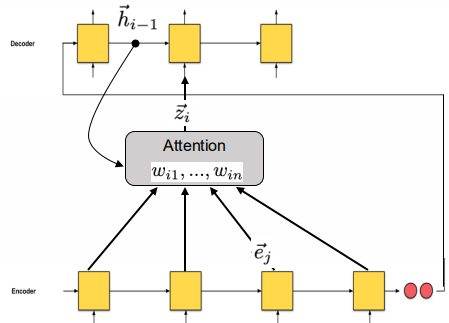
\includegraphics[width=0.5\linewidth]{images/nlp4.png}
    \caption{Attention}
\end{figure}

\paragraph*{Similarity}
There are two common methods for computing similarity between the decoder state and input embeddings:
\begin{itemize}
    \item \textit{Additive attention}: similarity is computed using a feed-forward neural network:
        \[\text{similarity}(\textbf{h}_{i-1},\textbf{e}_j)=\text{FFNN}(\textbf{h}_{i-1},\textbf{e}_j)\]    
    \item \textit{Multiplicative attention}: similarity is computed as the dot product between the decoder state and the input embedding, normalized by the square root of the embedding dimension $d$ to ensure stable gradients:
        \[\text{similarity}(\textbf{h}_{i-1},\textbf{e}_j)=\dfrac{\textbf{h}_{i-1}\cdot\textbf{e}_j}{\sqrt{d}}\]    
        Once the similarity weights are calculated, they are used to compute the weighted sum of the input embeddings:
        \[\textbf{z}_i=\sum_j\text{softmax}\left(\dfrac{\textbf{h}_{i-1}\cdot\textbf{e}_j}{\sqrt{d}}\right)\textbf{e}_j\]

\end{itemize}

\paragraph*{Query-key-value}
Attention can be generalized using the query-key-value framework:
\[\textbf{z}_i=\sum_jw_{ij}\textbf{v}_j =\sum_j\text{softmax}\left(\dfrac{\textbf{q}_{i}\cdot\textbf{k}_j}{\sqrt{d}}\right)\textbf{v}_j\]
\noindent Here:
\begin{itemize}
    \item \textit{Query} ($\textbf{q}_i$): represents what the model is looking for at position $i$.
    \item \textit{Key} ($\textbf{k}_j$): acts as an index to locate relevant information.
    \item \textit{Value} ($\textbf{v}_j$): contains the actual information stored at position $j$.
\end{itemize}
\noindent These components are typically transformed using learned linear projections:
\[\textbf{q}_i=\textbf{W}_q\textbf{h}_{i-1}\qquad\text{k}_j=\textbf{W}_k\textbf{e}_j\qquad\textbf{v}_j=\textbf{W}_v\textbf{e}_j\]
Here, $\textbf{W}_q,\textbf{W}_k,\textbf{W}_v\in\mathbb{R}^{n\times n}$
\begin{figure}[H]
    \centering
    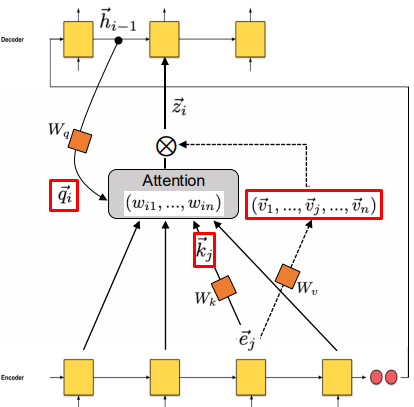
\includegraphics[width=0.5\linewidth]{images/nlp5.png}
    \caption{Query-key-value attention}
\end{figure}

\subsection{Self-attention}
Self-attention is a powerful mechanism that allows models to capture relationships between different parts of the input sequence without relying on recurrence or convolution.
Deeper models generally outperform shallow ones because each layer builds on simpler features extracted by the layers below. 
However, training RNNs poses significant challenges:
\begin{enumerate}
    \item Information must propagate from the first position of the encoder to the last position of the decoder, and gradient information must flow back along the entire sequence during backpropagation.
    \item RNNs process sequences sequentially, making parallelization difficult and resulting in training times that scale linearly with the length of the input ($\mathcal{O}(n)$). 
    \item Training deeper networks with many layers becomes increasingly difficult due to vanishing or exploding gradients.
\end{enumerate}
\noindent Self-attention addresses these issues by removing the recurrent connections from the encoder and decoder. 
Instead, it relies on attention mechanisms to directly pass information between positions in the sequence.

\paragraph{Problems}
Removing recurrence introduces two main challenges:
\begin{enumerate}
    \item \textit{Query choice}: the current output of the encoder is used as the query instead of relying on the decoder's context.
    \item \textit{Word order loss}: positional encoding is added to the input embeddings to explicitly encode the order of words.
\end{enumerate}

\paragraph*{Computation}
Self-attention updates a sequence of embedding vectors based on the weighted average of incoming embedding vectors. 
At each position $i$, the mechanism computes:
\begin{itemize}
    \item \textit{Query}: a linear transformation of the embedding at position $i$.
    \item \textit{Key}: a linear transformation of the embedding at position $j$.
    \item \textit{Value}: a linear transformation of the embedding at position $j$.
\end{itemize}
\noindent The output embedding at position $i$ is then computed as:
\[\textbf{z}_i=\sum_jw_{ij}\textbf{v}_j =\sum_j\text{softmax}\left(\dfrac{\textbf{q}_{i}\cdot\textbf{k}_j}{\sqrt{d}}\right)\textbf{v}_j\]

\paragraph{Applications}
Self-attention models are trained to perform tasks such as:
\begin{itemize}
    \item \textit{Masked Language Modeling}: recover missing words from the input text based on surrounding context.
        Input text is corrupted by randomly masking certain tokens, and the model learns to predict them.
    \item \textit{Next word prediction}: predict the next word in a sequence based on the previous words.
\end{itemize}